\section{Inledning}
\subsection{Teori \& bakgrund}
% Bakgrund

Automatiska växellådor sitter idag i en mängd av olika fordon,
däribland en helt elektrisk buss under utveckling av Volvo.
För att bland annat köra på rätt växel, optimera motorns styrprogram
och operera olika bromsfunktioner % och vad mer/något mer?
mätes fordonets lutning.
För det ändamålet ska lutningsgivare användas.
Lutningsgivaren är en fristående modul som kommunicerar med styrdatorn via
Controller Area Network (CAN)-kommunikation.
Detta fungerar bra vid rörelse i konstant hastighet
men vid accelereration uppstår mätbrus och andra störningar.
Därför behövs en algoritm för att felkompensera dessa störningar.

%teori
% - piezoelekrtiskakristaller
% - algoritmen

Piezoelektriska material, har en kristallstruktur och, ger upphov till
elektriska laddningar på dess yta under yttre mekaniskt tryck, den så kallade
direkta piezoelektriska effekten.
Det mekaniska arbete som utförs omvandlas till elektricitet, det omvända gäller
också, elektricitet omvandlas till mekansikt arbete i den omvända
piezoelektriska effekten i vilken kristallen deformeras.
\autocite{electronicdesign2016}
Piezoelektriska lutningsgivare använder elektriska signaler som är
inducerade via den piezoelektriska effekten från en piezoelektrisk kropp
under gravitationskraften från en tyngd.
Vinkeln mellan gravitationskraften och
riktningen på den piezoelektriska kroppens vibration
fås av att man mäter magnituden av kraftenkomponenten i vibrationens riktning
och använder geometriska samband mellan dem.
\autocite{chiang00}

%vad neuronnät är och vad de används till
Ett artificiellt neuronnät är ett en självlärande algoritm som inspirerats av
hur djurs hjärnor fungerar och kommunicerar.
Neuronnät kan användas för att klara av vissa problem som annars är svårlösta
med konventionella datalogiska metoder.
Ett neuronnät ``lär sig'', precis som vi gör, genom att observera.
Men för att ha avsedd funktion måste de tränas, alltså är arbete med neuronnät
uppdelat i två faser: en inlärningsfas och en tillämpningsfas där nätverket sedan
utför den ämnade uppgiften.
\autocite{copeland16}
Det är möjligt att sedan forstätta träna nätverket
under användning, men oftast slutar man träna det när resultet är önskvärt.
\autocite{wiki-neuronnat}

\def\layersep{2.5cm}
\begin{figure}
	\centering
	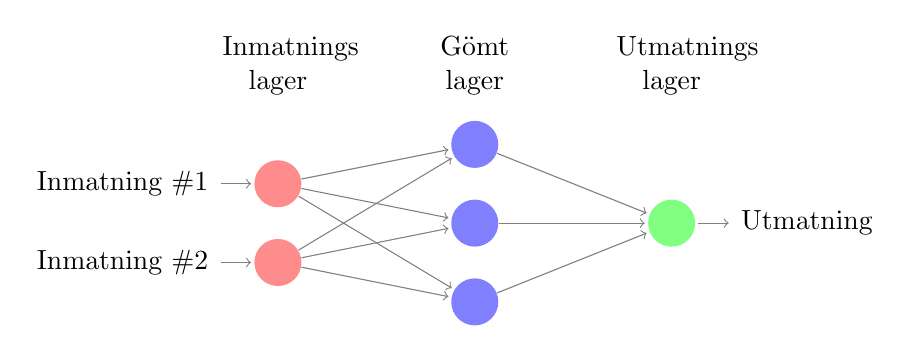
\begin{tikzpicture}[shorten >=1pt,->,draw=black!50, node distance=\layersep]
		\tikzstyle{every pin edge}=[<-,shorten <=1pt]
    	\tikzstyle{neuron}=[circle,fill=black!25,minimum size=17pt,inner sep=0pt]
    	\tikzstyle{inmatning}=[neuron, fill=red!45];
    	\tikzstyle{utmatning}=[neuron, fill=green!50];
    	\tikzstyle{hidden neuron}=[neuron, fill=blue!50];
    	\tikzstyle{annot} = [text width=4em, text centered]

    	\foreach \name / \y in {1,...,2}
        	\node[inmatning, pin=left:Inmatning \#\y] (I-\name) at (0,-\y) {};
    	\foreach \name / \y in {1,...,3}
        	\path[yshift=0.5cm]
            	node[hidden neuron] (H-\name) at (\layersep,-\y cm) {};
    	\node[utmatning,pin={[pin edge={->}]right:Utmatning}, right of=H-2] (O) {};
    	\foreach \source in {1,...,2}
        	\foreach \dest in {1,...,3}
            	\path (I-\source) edge (H-\dest);
    	\foreach \source in {1,...,3}
        	\path (H-\source) edge (O);

    	\node[annot,above of=H-1, node distance=1cm] (hl) {Gömt lager};
    	\node[annot,left of=hl] {Inmatnings lager};
    	\node[annot,right of=hl] {Utmatnings lager};
    \end{tikzpicture}
	\caption{Allmänt neuronnät}
	\label{fig:genericnetwork}
\end{figure}

% Williams personliga TODO:
%	- bli konsekvent i hur begrepp ska skrivas, alltså språk osv.
%	- knyt ihop styckena bra
%   - ska det vara med hur antal neuroner bestämms?
%   - recurrent
%	- skulle kanske vara vettigt med en mer utförlig förklaring av weights och
%	  biases

%neuronnäts arkitektur
Neuronnät har en generell arkitektur, se figur~\ref{fig:genericnetwork}, där
det lagret längst till vänster är inmatningslagret (bestående av
inmatningsneuroner), det längst till höger är utmatningslagret (bestående av
utmatningsneuroner). Det mellersta kallas det gömda lagret för att det varken
innehåller in- eller utmatningsneuroner. Varje neuron får sin inmatning från
varje annan neuron i det föregående lagret, förutom inmatningsneuronerna som
direkt får data. %rätt att använda data!?
Den här arkitekturen kallas \textit{feedforward}, inforamtionen matas
alltid framåt.
%sigmoid neuroner
Neuronnät består av s.k. sigmoidneuroner vars inmatning, $x$ är ett tal mellan 0 och 1.
Varje neuron är tilldelad en \textit{weight}, $w$, och en \textit{bias}, $b$.
Förenklat säger weighten av hur stor betydelse informationen är för neuronen
och biasen i hur hög grad man bör lita på denna enskilda neuron.
Utmatningen, $\sigma$, från en sigmoidneuron blir alltså: $ \sigma(w \cdot x
+b) $, där $\sigma$ kallas sigmoid funktionen, och defineras som:

\begin{equation}
	\sigma(z) \equiv \frac{1}{1 + e^{-z}} \\
\end{equation}

Utmatningen för en sigmoid neuron med inmatningen $ x_1, x_2,
\ldots$, weightsen $w_1, w_2, \ldots$ och biasen $b$ är:

\begin{equation}
	\frac{1}{1 + \exp(-\Sigma_jw_jx_j - b)}
\end{equation}

%skulle behöva fixa en förklaring av mina variabler

Tänk att $z \equiv w \cdot x + b $ och är ett stort positivt tal då är $e^{-z} \approx 0 $
medan $\sigma(z) \approx 1$.
Motsatt gäller att när $z$ är ett stort negativt tal går $e^{-z} \rightarrow
\infty $ och därmed $\sigma(z) \approx 0$. Det är alltså bara när talen är
stora som förändringen är drastiskt. Inom ramen för ``små'' tal ger de en
gradvis förändring, vilket går se på formen av sigmoid funktionen om man
visualierar den, se figur~\ref{fig:sigmoid}.

\begin{comment}
	Kolla så att det här faktiskt är rätt

Alltså kommer en liten förändring i en weight, $\Delta w_j$, eller bias,
$\Delta b_j$, att ge en liten förändirng i utmatningen,
$\Delta\text{utmatning}$:

\begin{equation}
	\Delta \mbox{utmatning} \approx \sum_j \frac{\partial \, \mbox{utmatning}}{\partial w_j}
	\Delta w_j + \frac{\partial \, \mbox{utmatning}}{\partial b} \Delta b,
\end{equation}

där summan betecknar de partiella derivatorna i förhållande till weights
respektive biases. Vilket innebär att $\Delta\text{utmatning}$ är
\end{comment}

\begin{figure}
	\centering
	\begin{tikzpicture}
		\begin{axis}[xlabel=$Z$,xmin=-5,xmax=5,]
			\addplot[red!75] {(1)/(1+e^-x)};
		\end{axis}
	\end{tikzpicture}
	\caption{Sigmoid funktion}
	\label{fig:sigmoid}
\end{figure}


% Förlustfunktionen
Med hjälp av en slät funktion för hur väl nätet approximerar träningsdatan
kan man korrelera små ändringar i weights och biases
till små förbättringar i prestandan.
Den \emph{kvadratiska förlustfunktionen} är en sådan funktion:

\begin{equation}
	C(w, b) \equiv \frac{1}{2n} \displaystyle\sum_x \lVert y(x) - a \rVert^2
\end{equation}

där $ w $ är alla weights i nätet, $ b $ är alla biases,
$ n $ är antalet träningsindata, $ a $ är en vektor med utdata när $ x $ är indata
och summan är över all träningsindata $ x $.
Man ser att $ C(w, b) $ är icke-negativ då varje term i summan är positiv.
Dessutom är förlusten $ C(w, b) $ liten, det vill säga $ C(w, b) \approx 0 $,
när $ y(x) $ är ungefär lika med utdatan, $ a $, för alla träningsindata, $ x $.
Målet med träningsalgoritmen blir då att minimera $ C(w, b) $.

\begin{figure}
	\centering
	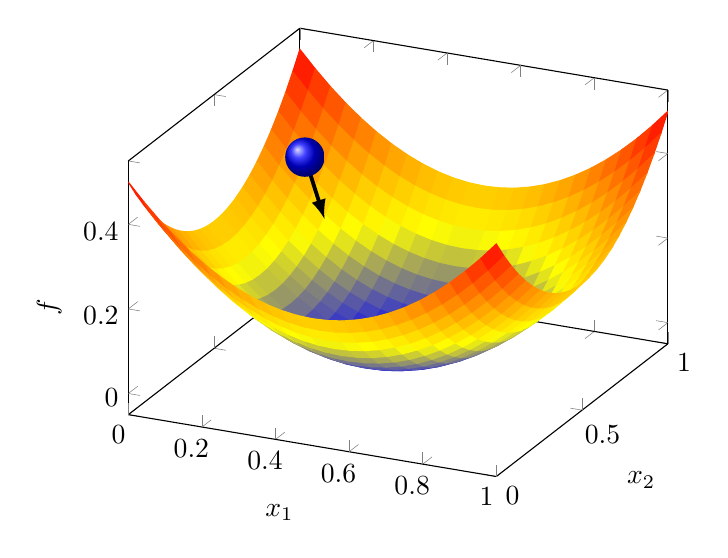
\begin{tikzpicture}
		\begin{axis}[domain=0:1,xlabel={$x_1$},ylabel={$x_2$},zlabel={$f$}]
			\addplot3[surf,shader=flat] {(x-0.5)^2 + (y-0.5)^2};
			\draw[->,line width=0.004\linewidth,>=latex] (axis cs:0.2,0.6,0.4) -- (axis cs:0.3,0.5,0.3);
			\node[circle,shading=ball,minimum width=0.5cm] (ball) at (axis cs:0.2,0.6,0.4) {};
		\end{axis}
	\end{tikzpicture}
	\caption{Gradient descent}
	\label{fig:descent}
\end{figure}

En algoritm för det är \emph{gradient descent}.
Om man föreställer sig en funktion $ f(x_1, x_2) $ som en dal,
se figur~\ref{fig:descent},
säger intuition att en boll skulle rulla ner för sluttningen till botten.
Vi kan simulera detta genom att räkna ut gradienten av $ f $.
Gradienten av $ f $, $ \nabla f $, vid en punkt är en vektor
som pekar i riktningen av den brantaste lutningen vid den punkten:

\begin{equation}
	\nabla f = \begin{bmatrix} \frac{\partial f}{\partial x_1} & \frac{\partial f}{\partial x_2} \end{bmatrix}^{T}
\end{equation}

där $ \partial f / \partial x_i $ är den partiella derivatan
som beskriver hur snabbt $ f $ växer med avseende på variablen $ x_i $.
Vi kan minska $ f $ genom att gå i riktningen av den negativa gradienten:

\begin{equation}
	x \rightarrow x' = x - \eta \nabla f(x)
\end{equation}

där $ \eta $ är inlärningshastigheten,
en positiv skalär som bestämmer längden av steget.

\subsection{Syfte}
Syftet med undersökningen är att ta fram och utvärdera en algoritm med
artificiella neuronnät som felkompenserar lutningsgivare i elbussväxellådor.

\subsection{Frågeställningar}
Vi vill undersöka\ldots
\begin{itemize}
	\item Varför råsignalen från lutningsgivaren blir opålitlig.
	\item Hur nätverket ska vara konfigurerat för att felkompensera; vilka inputs,
		outputs, antal neuroner, hidden layers och feed-/cascade-forward?
	\item Hur väl det fungerar att felkompensera med neuronnät.
\end{itemize}
